\section{Dispositivos de proteção}

\begin{frame}{Introdução}
	\begin{block}{}
		\begin{itemize}
			\item Imagine um \textbf{acidente elétrico natural} como, por exemplo, um \textbf{raio}, ou \textbf{trovão}.
			\item Esses fenômenos podem causar \textbf{sérios danos} aos nossos eletrodomésticos.
			\item Felizmente, é possível evitar esses problemas com a instalação de \textbf{dispositivos de proteção}.
		\end{itemize}
	\end{block}

	\centering
	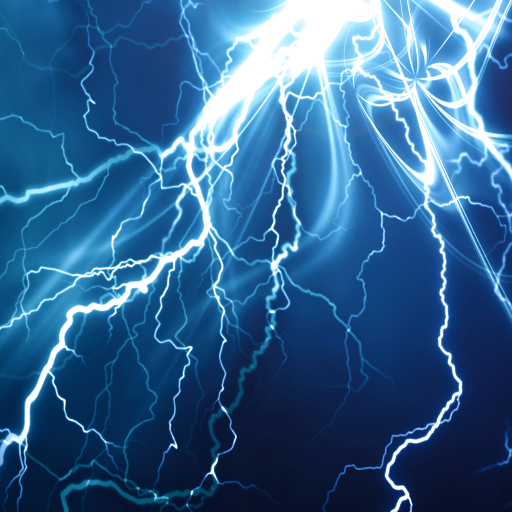
\includegraphics[height=0.5\textheight]{Figuras/Ch04/fig11}

\end{frame}



\begin{frame}{Introdução}
	\begin{block}{Noções iniciais}
		\begin{itemize}
			\item Os fusíveis e disjuntores são \textbf{equipamentos elétricos} que atuam \textbf{automaticamente} pela ação de \textbf{dispositivos sensíveis}.
			\item Quando o \textbf{circuito elétrico} ao qual estão \textbf{conectados} se encontra submetido a determinadas \textbf{condições anormais} eles \textbf{seccionam} a \textbf{conexão} com a \textbf{fonte de tensão}.
			\item Isso tem o objetivo de \textbf{evitar} ou \textbf{limitar} os \textbf{danos} a um \textbf{sistema} ou \textbf{equipamento elétrico}.
			\item Os \textbf{principais dispositivos de proteção} utilizados em \textbf{instalações prediais} são:
			      \begin{itemize}
				      \item\normalsize disjuntores termomagnéticos;
				      \item\normalsize disjuntores diferenciais, e;
				      \item\normalsize fusíveis.
			      \end{itemize}
		\end{itemize}
	\end{block}
\end{frame}


\begin{frame}{Disjuntor x Fusível}
	\begin{block}{}
		\begin{itemize}
			\item Você sabe a diferença entre um \textbf{fusível} e um \textbf{disjuntor}?

		\end{itemize}
	\end{block}

	\bigskip

	\centering
	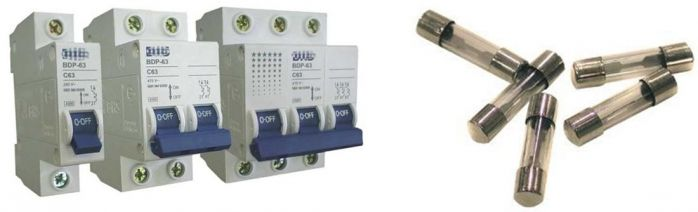
\includegraphics[width=1\linewidth]{Figuras/Ch04/fig6}
\end{frame}


\begin{frame}{Disjuntor x Fusível}
	\begin{block}{Noções iniciais}
		\begin{itemize}
			\item Os dois são usados para \textbf{proteção contra sobrecorrente }em circuitos.
			\item Toda vez que a rede de alimentação dá \textbf{picos}, ou que uma tomada é \textbf{mal utilizada} (e, portanto, há \textbf{sobrecarga}), ou no caso de \textbf{curtos-circuitos} (quando a resistência é \textbf{nula}) há \textbf{sobrecorrente}.
			\item Esses equipamentos protegem contra a sobrecorrente, porém de formas \textbf{distintas}.
		\end{itemize}
	\end{block}

	%	\centering
	%	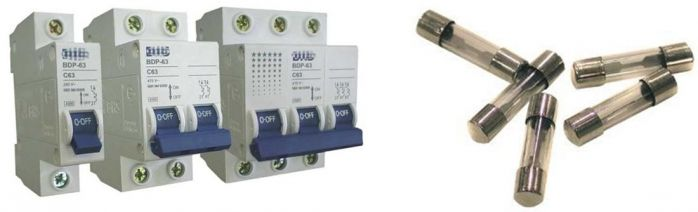
\includegraphics[width=0.7\linewidth]{Figuras/Ch04/fig6}
\end{frame}


\begin{frame}{Disjuntor x Fusível}
	\begin{block}{Fusível}
		\begin{itemize}
			\item O fusível é um \textbf{fio não isolado} cuja bitola é calculada para que, com a ocorrência de \textbf{sobrecorrente}, ele se esquente o suficiente para se \textbf{partir imediatamente}.
			\item Isso diminui muito o \textbf{risco de danos} à equipamentos posteriores.
			\item O fusível é de \textbf{uso único}, ou seja, uma vez queimado, necessita ser \textbf{reposto}.
		\end{itemize}
	\end{block}

	%	\centering
	%	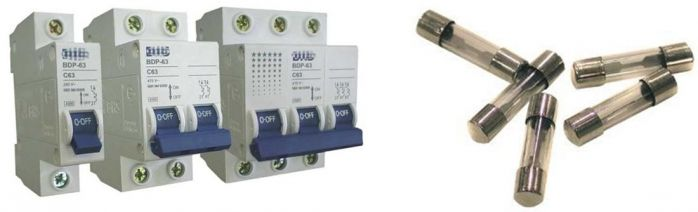
\includegraphics[width=0.7\linewidth]{Figuras/Ch04/fig6}
\end{frame}


\begin{frame}{Disjuntor x Fusível}
	\begin{block}{Disjuntor}
		\begin{itemize}
			\item Já o disjuntor não é de uso único e \textbf{pode ser religado} depois que as anomalias na rede forem resolvidas.
		\end{itemize}
	\end{block}

	\centering
	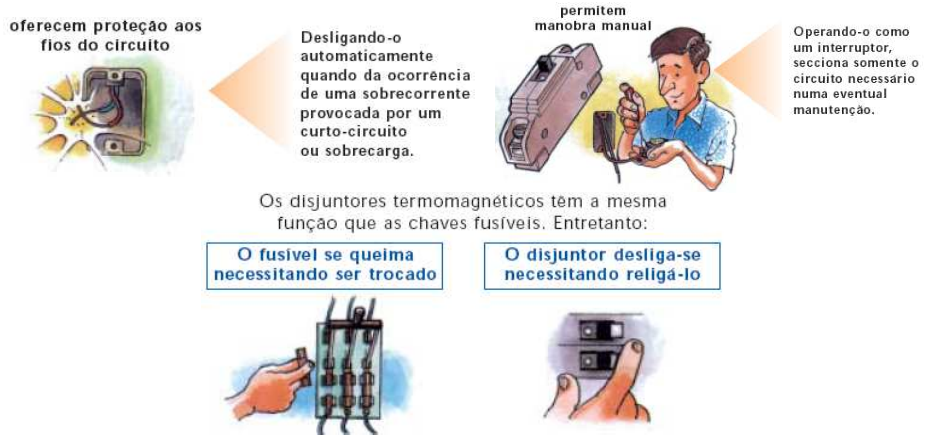
\includegraphics[width=1\linewidth]{Figuras/Ch04/fig1}
\end{frame}


\begin{frame}{Disjuntor}
	\begin{block}{Tipos}
		O disjuntor pode ser de três tipos:
		\begin{itemize}
			\item Térmico
			\item Magnético
			\item Termomagnético (mais utilizado)
		\end{itemize}
	\end{block}

	\vspace{0.25cm}

	\begin{minipage}{0.3\linewidth}
		\centering
		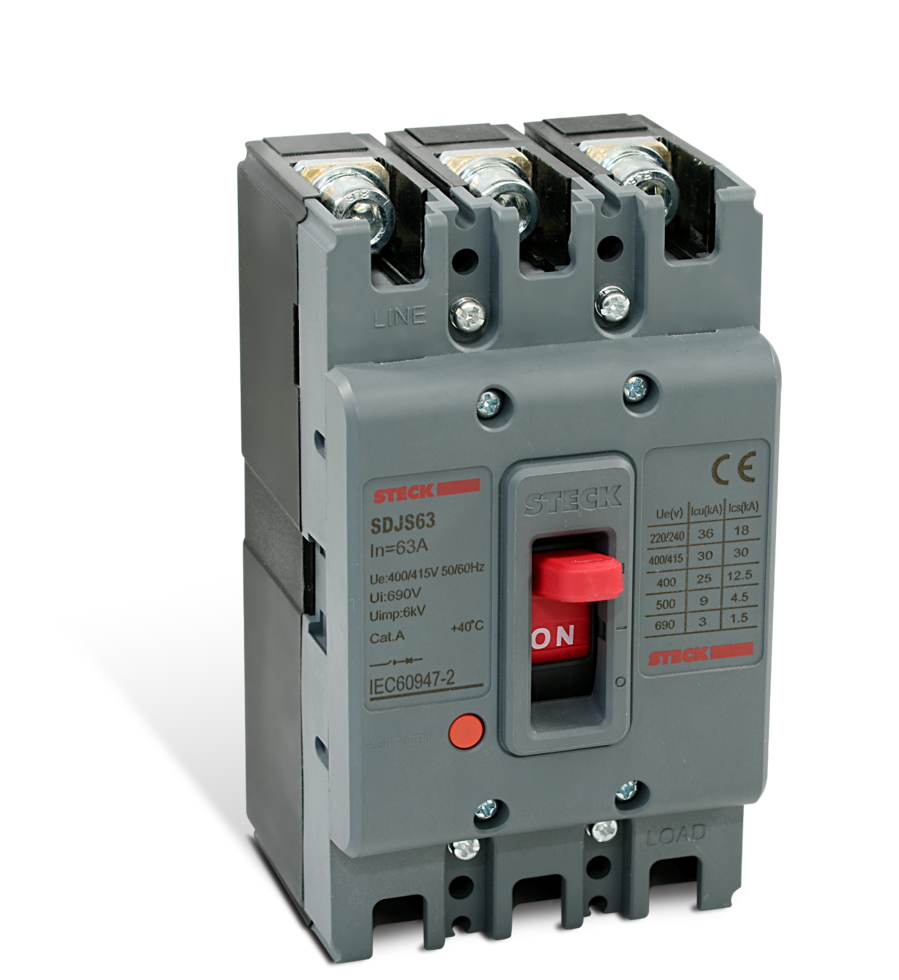
\includegraphics[width=1\linewidth]{Figuras/Ch04/fig7}
	\end{minipage}\hfill
	\begin{minipage}{0.3\linewidth}
		\centering
		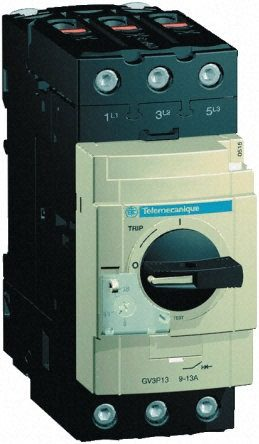
\includegraphics[width=0.6\linewidth]{Figuras/Ch04/fig8}
	\end{minipage}\hfill
	\begin{minipage}{0.3\linewidth}
		\centering
		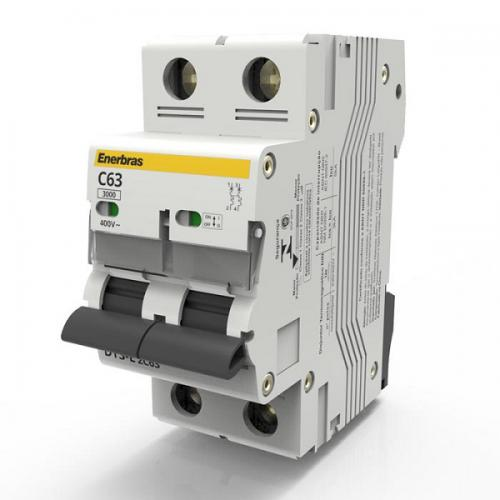
\includegraphics[width=1\linewidth]{Figuras/Ch04/fig9}
	\end{minipage}
\end{frame}


\begin{frame}{Disjuntor Térmico}
	\begin{block}{Características}
		\begin{itemize}
			\item Funcionam através da deformação de uma \textbf{lâmina bimetálica}:
			      quando ocorre uma \textbf{sobrecarga} e a corrente elétrica neste disjuntor é \textbf{maior que a aceitável}, a \textbf{lâmina bimetálica} se \textbf{aquece} e começa a se \textbf{deformar}, esta deformação \textbf{abre o contato}, seccionando o circuito protegido.
		\end{itemize}
	\end{block}

	\centering
	\begin{tikzpicture}[x=1.2cm,y=1.2cm]
		\fill[pattern=north east lines] (0,0) rectangle +(-0.5,2);
		\draw (0,0) -- (0,2);
		\draw (0,1.2) -- ++(3,0) -- ++(0,-0.2) -- +(-3,0) (0,0.8) -- ++(3,0) -- +(0,0.2);
		\fill[pattern=north west lines] (0,0.8) rectangle +(3,0.2);
		\node at (1.5,1.4) {\small A};
		\node at (1.5,0.6) {\small B};
		\node(A) at (2,0) {};
		\node(B) at (2,2) {};
		\draw[->,>=Latex] (A) edge[bend right] (B);
	\end{tikzpicture}
\end{frame}


\begin{frame}{Disjuntor Térmico}
	\begin{block}{Características}
		\begin{itemize}
			\item É um componente mecanicamente \textbf{simples} e \textbf{robusto}.
			\item É relativamente \textbf{barato}.
			\item \textbf{Não} possui grande \textbf{precisão} de corrente de seccionamento.
			\item É usado apenas para \textbf{aquecimentos de longo prazo}, não sendo possível o seu uso para proteção contra curto-circuitos ou sobrecorrente de pico.
		\end{itemize}
	\end{block}

	\centering
	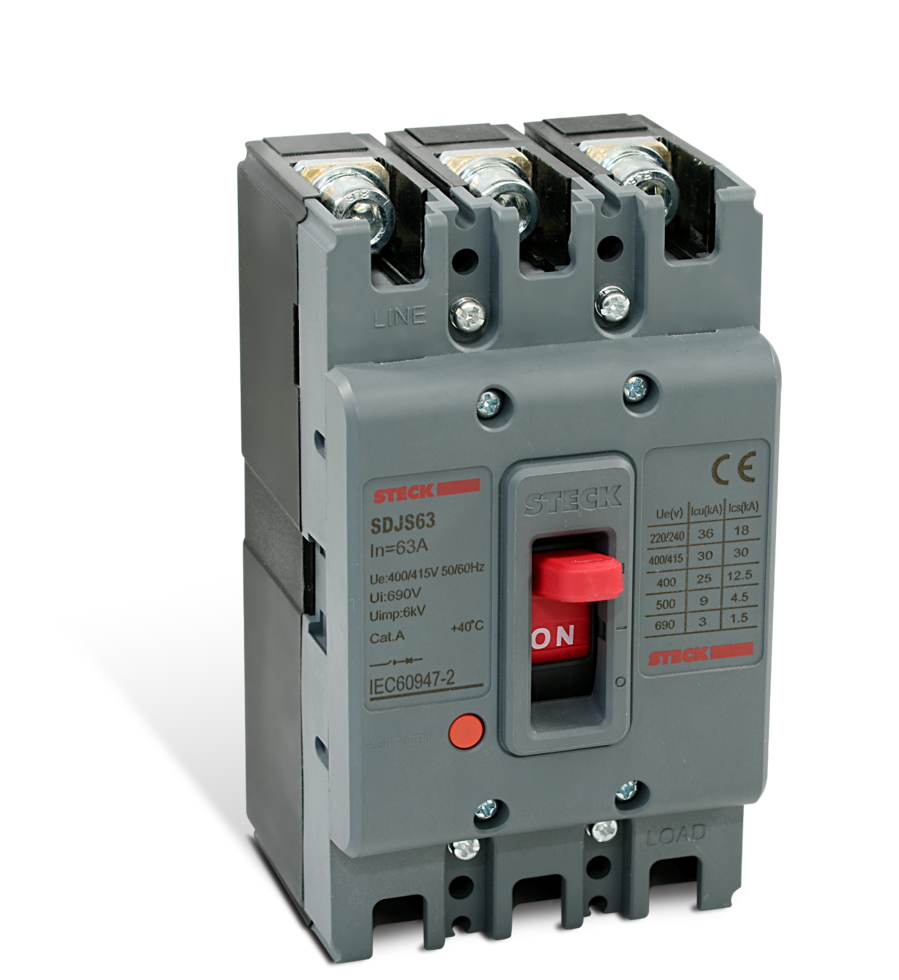
\includegraphics[height=0.4\textheight]{Figuras/Ch04/fig7}
\end{frame}


\begin{frame}[fragile]{Disjuntor Magnético}
	\begin{block}{Características}
		\begin{itemize}
			\item Quando há uma \textbf{variação de corrente} passando por um \textbf{fio}, um \textbf{campo magnético} é \textbf{induzido}.
			\item Partindo disso, podemos dimensionar uma bobina que, quando percorrida por uma \textbf{forte} corrente elétrica \textbf{desloca um contato}, seccionando, assim, um circuito.
			\item Como o efeito é praticamente instantâneo, podemos substituir o fusível por um disjuntor termomagnético.
		\end{itemize}

	\end{block}

	\begin{minipage}{0.45\linewidth}
		\centering
		%		\scalebox{0.95}{
		\begin{tikzpicture}
			% 1.5 ... radius of the rings
			% 0.3 ... how far the rings are apart
			% 0.4 ... how much from the side the rings are seen (try 0 and the same as the radius)
			\def\coil#1{
				{-2.5mm * cos(\t * pi r)+14},
				{0.15 * (2*#1 + \t) + 0.1*sin(\t * pi r)+0.67}
			}

			%			\draw[decoration={aspect=0.3, segment length=3mm, amplitude=3mm,coil},decorate] (0.5,0.8) -- (0.5,2);
			% coil behind the rectangle
			\foreach \n in {1,2} {
					\draw[domain={0:1},smooth,variable=\t,samples=15]
					plot (\coil{\n});
				}

			\draw[domain={0:0.5},smooth,variable=\t,samples=15] plot (\coil{3});

			% Draw the rectangle
			\filldraw[fill=white,draw=black] (0.3, 0) rectangle (0.7, 1.5);

			%	coil in front of the rectangle
			\foreach \n in {1,2} {
					\draw[domain={1:2},smooth,variable=\t,samples=15]
					plot (\coil{\n});
				}

			\draw[domain={1.5:2},smooth,variable=\t,samples=15] plot (\coil{0});


			\draw (-1,0.5) -- (0.5,0.5) -- +(0,0.3) (-1,2) -- (0.5,2) -- (0.5,1.75);
			\draw[->,>=Latex] (-1,2.1) -- +(0.5,0) node[above] {$ i $};
			\draw[->,>=Latex] (-1,0.1) -- +(0.5,0) node[above] {$ i $};
			\draw (0.5, 0.3) -- +(1,0.5) node[right] {barra metálica};
			\draw (-1,0) -- (0,0)
			node[circle,fill=black,inner sep=1] {} -- (1,0) node[circle,fill=black,inner sep=1] {} -- (2,0);
		\end{tikzpicture}
		%		}
	\end{minipage}
	\hfill
	\begin{minipage}{0.45\linewidth}
		\centering
		%		\scalebox{0.95}{
		\begin{tikzpicture}
			% 1.5 ... radius of the rings
			% 0.3 ... how far the rings are apart
			% 0.4 ... how much from the side the rings are seen (try 0 and the same as the radius)
			\def\coil#1{
				{-2.5mm * cos(\t * pi r)+14},
				{0.15 * (2*#1 + \t) + 0.1*sin(\t * pi r)+0.67}
			}

			%			\draw[decoration={aspect=0.3, segment length=3mm, amplitude=3mm,coil},decorate] (0.5,0.8) -- (0.5,2);
			% coil behind the rectangle
			\foreach \n in {1,2} {
					\draw[domain={0:1},smooth,variable=\t,samples=15]
					plot (\coil{\n});
				}

			\draw[domain={0:0.5},smooth,variable=\t,samples=15] plot (\coil{3});

			% Draw the rectangle
			\filldraw[fill=white,draw=black] (0.3, 0.35) rectangle (0.7, 1.85);

			%	coil in front of the rectangle
			\foreach \n in {1,2} {
					\draw[domain={1:2},smooth,variable=\t,samples=15]
					plot (\coil{\n});
				}

			\draw[domain={1.5:2},smooth,variable=\t,samples=15] plot (\coil{0});


			\draw (-1,0.5) -- (0.5,0.5) -- +(0,0.3) (-1,2) -- (0.5,2) -- (0.5,1.85);
			\draw[->,>=Latex] (-1,2.1) -- +(0.5,0) node[above] {$ i^\prime $};
			%			\draw (0.3, 0.35) rectangle (0.7, 1.85);
			\draw (-1,0) -- (0,0)
			node[circle,fill=black,inner sep=1] {} -- (1,0.5) node[circle,fill=black,inner sep=1] {} (1,0) -- (2,0);
		\end{tikzpicture}
		%		}
	\end{minipage}
\end{frame}


\begin{frame}{Disjuntor Termomagnético}
	\begin{block}{Características}
		\begin{itemize}
			\item Os disjuntores termomagnéticos reúnem \textbf{ambos} mecanismos, sendo \textbf{os mais utilizados}.
			\item Os tipos de disjuntores termomagnéticos existentes no mercado são: monopolares, bipolares e tripolares.
			\item Os disjuntores termomagnéticos somente devem ser ligados aos \textbf{condutores fase} dos circuitos.
		\end{itemize}

	\end{block}

	\centering
	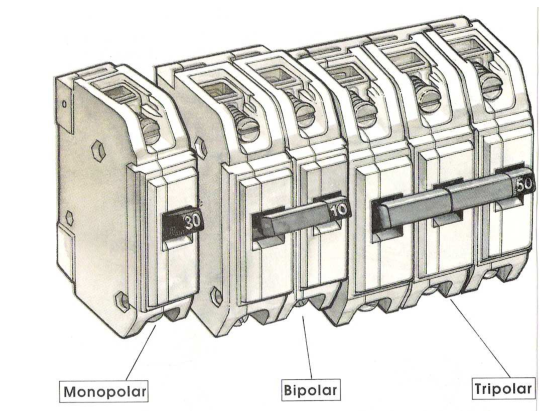
\includegraphics[width=0.45\linewidth]{Figuras/Ch04/fig2}
\end{frame}


%\begin{frame}{Disjuntor Termomagnético}
%	\begin{block}{Características}
%		\begin{itemize}
%			\item Os tipos de disjuntores termomagnéticos existentes no mercado são: monopolares, bipolares e tripolares.
%			\item Os disjuntores termomagnéticos somente devem ser ligados aos condutores fase dos circuitos.
%		\end{itemize}
%		
%	\end{block}
%
%	\centering
%	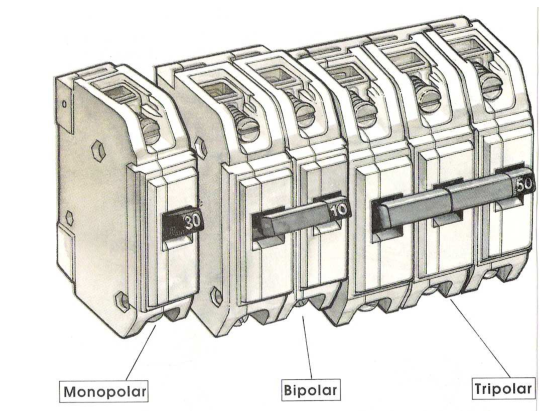
\includegraphics[width=0.5\linewidth]{Figuras/Ch04/fig2}
%\end{frame}


\begin{frame}{Disjuntor Diferencial Residual}
	\begin{block}{Características}

		\begin{itemize}
			\item É um dispositivo constituído de um disjuntor termomagnético acoplado a um outro dispositivo: o diferencial residual.
		\end{itemize}
	\end{block}

	\centering
	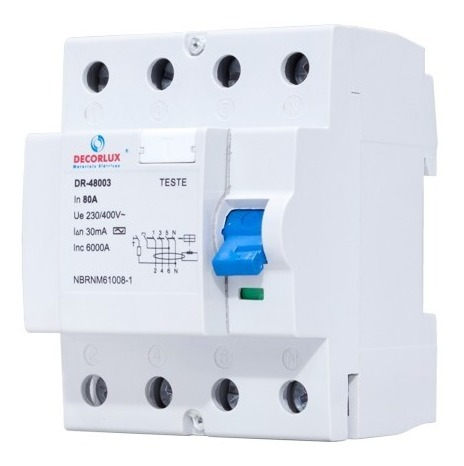
\includegraphics[width=0.4\linewidth]{Figuras/Ch04/fig10}
\end{frame}


\begin{frame}{Disjuntor Diferencial Residual}
	\begin{block}{Dispositivo Diferencial Residual}

		\begin{itemize}
			\item O dispositivo Diferencial Residual, ou DR, é um dispositivo de \textbf{segurança} utilizado em instalações elétricas.
			\item Sua função é detectar pequenas \textbf{fugas de corrente} em circuitos elétricos, acionando o desligamento imediato da alimentação e evitando que ocorram acidentes.
			\item Essas fugas podem acontecer por diferentes razões: um \textbf{toque} acidental, um fio \textbf{desencapado}, o uso de equipamentos elétricos em áreas \textbf{molhadas} ou até mesmo um brinquedo que foi inserido na tomada por uma criança.
			\item Em situações como estas, a corrente elétrica corre para a terra \textbf{através do corpo humano}, causando \textbf{acidentes} com choque elétrico.
			      %			\item Um circuito inteiro não deve ser afetado caso outro apresente alguma falha. Desse modo, o DR torna-se o meio mais eficaz na proteção de pessoas e animais domésticos, evitando que ocorram acidentes.
			\item O dispositivo também protege contra incêndios.
		\end{itemize}
	\end{block}

	%	\centering
	%	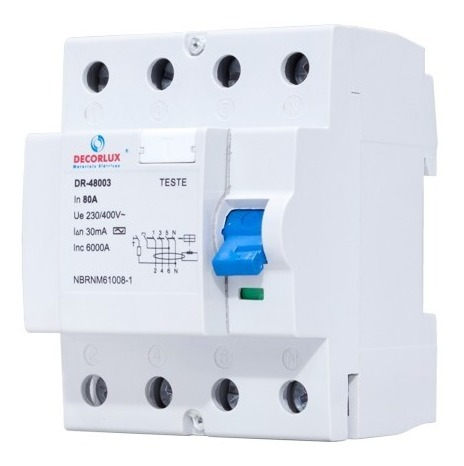
\includegraphics[width=0.4\linewidth]{Figuras/Ch04/fig10}
\end{frame}


\begin{frame}{Disjuntor Diferencial Residual}
	\begin{block}{Características}

		\begin{itemize}
			\item Desta forma o disjuntor diferencial é um dispositivo que protege os fios do circuito contra sobrecarga e curto-circuito e as pessoas contra choques elétricos.
		\end{itemize}
	\end{block}

	\centering
	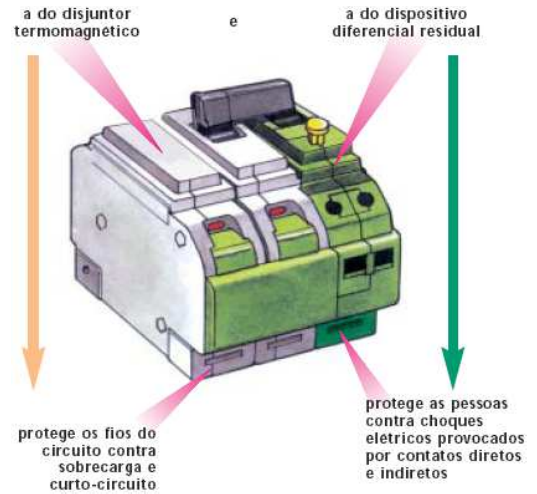
\includegraphics[width=0.5\linewidth]{Figuras/Ch04/fig3}
\end{frame}


\begin{frame}{Interruptor Diferencial Residual}
	\begin{block}{Características}
		\begin{itemize}
			\item É um dispositivo constituído de um interruptor acoplado a um diferencial residual.
		\end{itemize}

	\end{block}

	\centering
	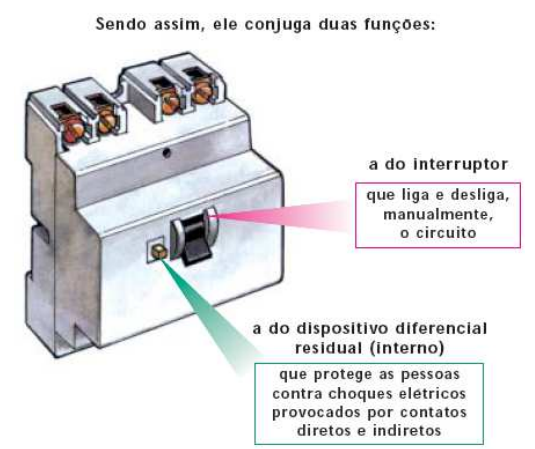
\includegraphics[width=0.45\linewidth]{Figuras/Ch04/fig4}
\end{frame}


\section*{Exercícios}
\frame{
	\frametitle{Exercícios}
	\begin{block}{}
		01. Descreva a diferença entre um fusível e um disjuntor com suas próprias palavras.

		\bigskip

		02. Como você faria a instalação elétrica da sua casa? Esboce um esquema.
	\end{block}
}

\section*{Referências}

\frame{
	\frametitle{Referências e Exercícios Complementares}
	\begin{itemize}
		\item CREDER, Hélio; Instalações Elétricas, 14ª edição, Editora LTC, Rio de Janeiro, 2004.
		\item Manual de Instalações Elétricas - Prysmian.
	\end{itemize}
	%\centering{\alert{Página 36 - \textbf{1.6.1 até 1.6.5, 1.6.17 até 1.6.19}}} \\
	%	\centering{\alert{Lista de exercícios 01}}
}